\documentclass[10pt,a4paper]{article}

\bibliographystyle{ieeetr}

\usepackage[margin=1in]{geometry}
\usepackage{graphicx}
\usepackage{subfig}
\usepackage{amsmath}
\usepackage{url}
\usepackage{pgfgantt}
\usepackage{lscape}
\usepackage{pdfpages}
\usepackage[title]{appendix}
% \usepackage{diagbox}

\graphicspath{{./figs/}}

\newcommand{\code}[1]{\texttt{#1}}

\title{A modular kernel for the Raspberry Pi: Progress Report}

\begin{document}

\maketitle

\begin{center}
    Thomas Archbold \\
    1602581 \\
    University of Warwick \\
\end{center}

\section{Introduction}
% problem that project addresses, motivations (importance of undertaking)
% make sure objectives are clear and clarify why it is a significant undertaking
% and of suitable level for third year project in computer science

\section{Background}
% all research I have put into it until this point - good understanding of
% background and how it fits into landscape (does not exist in isolation, before
% or after conception)
% indication of how background information was gained - a few citations that
% have been key sources for project

\section{Current progress}
The project is currently at a point at which the operating system is able to
successfully boot in the emulated environment provided by QEMU. Since it has
been capable of doing this since \code{boot.s} was written, early on in Term 1,
it is important to note the specific stages of initialisation performed by the
kernel at this point, as well as discuss the environment setup that has enabled
this point in development to be reached.

\subsection{Development environmet}
The project is being developed on a machine running Linux kernel version 4.16
onwards. Since the target environment, the Raspberry Pi 2 Model B, is different
to that on which it is being developed, a cross-compiler is required to compile
code that will run on the target machine, as opposed to the host. In particular,
available for download on the ARM developer website \cite{GNUtoolchain} is the
GNU Embedded Toolchain, which provides tools to target ARM Cortex family of
processors, including the GNU Compiler Collection (GCC). Conveniently this suite
of tools is available from Arch Linux's package manager, pacman \cite{pacman},
and this is the version of the cross-compiler used in the makefile.

Before writing any code, as the author had little-to-no prior experience in
systems programming, research had to be undertaken in order to get acquainted
with this environment. In particular, this involved skimming over the various
peripherals manuals, technical reference manuals, and programmer's guides for
programming on the Raspberry Pi to learn more about its hardware and how to
interface with it using ARM assembly. \cite{BCM2835} and \cite{BCM2836} detail the
peripherals on board the Raspberry Pi 2 Model B, the layout of their related
registers, and how to read and write them to do meaningful things with the
hardware, while \cite{TRM} and \cite{PG} provided help on ARM assembly's syntax,
and how and when to use specific instructions.

Particularly important so far have been the sections of the peripherals manual
on GPIO and UART, as until the implementation for the mailbox interface is
working, all input and output is done through the serial connection provided by
the UART.  Since there were issues with getting the Pi to run on real hardware,
information about the GPIO peripheral was needed in order to write basic
low-level debugging functions, mainly in the form of getting the green ACT LED
to blink for various return values of functions.

\subsection{boot.s}
The first piece of code to be written was \code{boot.s}, which is responsible
for providing the basic setup of the entire system, which includes initialising
a minimum C environment. In particular, it sends three of the four cores on the
CPU to shutdown (to decrease overall complexity of the system, as discussed in
the specification), initialises the stack pointer at address \code{0x8000}, sets
up the BSS segment (where statically-allocated variables that are not explicitly
initialised are stored) and zeroes it out (as required by the C standard), and
then loads our C kernel entry point, \code{kernel\_main}, into memory to begin
its execution. Note that the Program Counter for the kernel starts at address
\code{0x8000} and grows upwards, so the stack can safely start at \code{0x8000}
without interfering with the kernel (as it grows downwards).

\subsection{linker.ld}
The code in \code{linker.ld} is responsible for linking all of the compiled
object files into one final executable. There are scripts which do this for
user-space programs, but since we are our own user-space, being the kernel, we
have to create one for ourselves. The various sections that the script defines
are as follows:
\begin{itemize}
    \itemsep0em
    \item \code{.text} - contains executable code
    \item \code{.rodata} - read-only data i.e. global constants
    \item \code{.data} - global variables initialised at compile-time
    \item \code{.bss} - uninitialised global variables
\end{itemize}

We also define the entry point of our entire operating system in this script,
namely the \code{\_start} routine from \code{boot.s}. This script also sets the
symbols \code{\_\_start} and \code{\_\_text\_start} to be \code{0x8000}, which
is where the bootloader will put the kernel image - the code from \code{boot.s}
will be put in the first part of this section, \code{.text.boot}. We use
\code{KEEP} to tell the compiler not to try to optimise the code in
\code{.text.boot}, and \code{ALIGN} sets the current address to the next
available page (the next address divisible by 4096). The \code{,rodata},
\code{.data}, and \code{.bss} sections are then declared in much the same way.

\subsection{Makefile}
The makefile was written to speed up the build process, and there are only a few
features to note. First is that here we specify that we are using the
\code{arm-none-eabi} toolchain, for the compiler to target the Raspberry Pi's
architecture as opposed to our own, in particular the Cortex-A7 processor. The
\code{-fpic} compilation flag is currently being used while we are ignoring the
Memory Management Unit, and in particular virtual memory, on the Pi, as it
creates position-independent code, and will keep separate applications from
interfering with each other within this single address space when processes are
implemented. The \code{-ffreestanding} compiler and linker flag, and the
\code{-nostdlib} linker flag, specifies that we are writing code in a
freestanding environment, and as such do not expect much of the C standard
library to exist, or for program startup to necessarily to be at \code{main()}.
Specifically, we only have access to the following header files:
\code{<float.h>}, \code{<iso646.h>}, \code{<limits.h>}, \code{<stdalign.h>},
\code{<stdarg.h>}, \code{<stdbool.h>}, \code{<stddef.h>}, \code{<stdint.h>}, and
\code{<stdnoreturn.h>}. The rest of the standard library must be implemented
ourselves.

\subsection{Atags}
The first piece of meaningful setup that can be done when the kernel is booted
is to get information about the memory available to the system. On the Raspberry
Pi, the bootloader creates creates a list of information about the hardware
called Atags, places it at address \code{0x100}, and passes it as the third
parameter to \code{kernel\_main} in register 2. Each tag in the list contains a
header consisting of two unsigned 32-bit values: the size of the tag (in 32-bit
words), and the tag value. Each header is then followed by information specific
to that tag, aside from \code{ATAG\_NONE}, which has no associated data, and
\code{ATAG\_CORE}, whose data is optional. To access the information in each of
the tags when we come across them, we must match the layout of each of the tags
\cite{atags} by defining appropriate C structs in \code{atag.h}.

To find the amount of memory on the device, we can skip through the Atags list
(using pointer arithmetic and information about the tag's size in its header)
until we come across the \code{ATAG\_MEM} tag. Then it is simply a case of
return the value in the \code{size} field of the \code{atag\_mem} struct.

\subsection{Organising memory}
Throughout the operating system's execution, different processes will require
memory to perform computations. Although the only thing doing anything
meaningful at the moment is the kernel, which can theoretically use any memory
it wants, in order to impose some order for later implementations of processes
and user space, we split the available memory up into 4KiB pages. The total
number of pages is therefore given by the total amount of memory divided by the
page size.

To organise the pages, we give each page a header which stores metadata about
the page, including whether the page has been allocated, whether it is a kernel
page, and whether this page is part of the heap (used later when dynamically
allocating memory). We organise all of the page headers into a linked list
directly after the end of the kernel image, using the \code{\_\_end} variable
from the linker script. Each page also stores the virtual address to which it
maps; as virtual memory has not yet been implemented, a page's virtual address is
simply its index in the page list multiplied by the page size. All that remains
is to iterate over the page header list to initialise each page's metadata, and
add each page to a linked list of all the free pages.

Naturally the next feature implemented was allocating and freeing pages.
Allocating a page is done by simply popping the head of the free page list,
setting the appropriate flags, and returning the address of the page. Freeing,
meanwhile, is done by passing the address of the page to free, again setting the
appropriate flags, and appending this page back to the fre page list.

\subsection{Allocating memory}
A 1MiB portion of memory located directly after the page headers is reserved for
the heap - while the choice of 1MiB is fairly arbitrary, it should be large
enough to suffice for all dynamic memory needs, and small enough to not use a
significant portion of memory that may be desired by user code. We define the
struct \code{heap\_segment} for keeping track of heap allocations, such as the
segment size and whether it has been allocated (useful for avoiding external
fragmentation later), and initialise the heap by declaring a single heap segment
whose size is equal to that of the heap - as more memory is allocated, this
initial segment will be split into smaller ones, which in turn may be split
further to satisfy requests for differing amounts of memory. Whenever memory is
requested, we add the size of the header to the request and 16-byte align it, so
as to actually reserve some space for the heap segment metadata.

To allocate a segment, we step through the list of segments in the heap and look
for the one best satisfying the number of bytes requested, and not in use. If
the current segment is large (i.e. the segemnt size if $\ge2$ times the header
size), we split it into two segments and only use one of them. Once a segment
satisfying the request is found, we return a pointer to the memory directly
after the header. To free an allocation, we set the appropriate flags, and then
attempt to merge consecutive free segments, checking both to the left and the
right of the current segment.

\subsection{Serial output}
Initial output was done using the UART on board the Pi, meaning text was sent
and received through serial ports. This was mainly due to simplicity in early
builds of the system, and while this can be achieved in the final version of the
project by using a USB-to-TTL cable, ideally it will use the HDMI port on the Pi
instead, which requires interfacing with the Mailbox peripheral (discussed
later). This was all done by interacting with the GPIO pins on the Pi, which is
done entirely through Memory Mapped I/O (MMIO) - that is, by reading from and
writing to predefined memory addresses. A peripheral on the Raspberry Pi is
simply an address to and from which you may read and write data, and all may be
described by an offset from the Peripheral Base Address; this is
\code{0x3f200000} on the Raspberry Pi 2 Model B. Moreover, a register is a
32-bit chunk of memory that a peripheral may read from or write to. The BCM2835
Peripherals Manual gives the UART base address as \code{0x7e201000}. Thus, in
\code{gpio.c}, after setting all the required flags for using the UART, we can
implement a serial \code{putc()} by checking that the FIFO is not full and
writing our data to the Data Register, and \code{getc()} by checking that the
FIFO is non-empty and reading from it. \footnote{From the manual: ``Physical
addresses range from \code{0x20000000} to \code{0x20ffffff} for peripherals. The
bus addresses for peripherals are set up to map onto the peripheral bus address
range starting at \code{0x7e000000}. Thus a peripheral listed at
\code{0x7ennnnnn} will be available at physical address \code{0x20nnnnnn}."}

\subsection{HDMI output}
The final goal, however, is to not use any extra adapters to make serial output
work - instead, output will be through the HDMI port on the Pi and to do so,
familiarisation with the Mailbox peripheral has been important. The Mailbox is a
peripheral that facilitates communication between the ARM CPU and the VideoCore
GPU \cite{Mailboxes}, and starts at offset \code{0xb880}. We may get data from the GPU via the
read register, pass data to the GPU using the write register, and check if
either of these are empty or full using the status register, at offsets
\code{0x00}, \code{0x20}, and \code{0x18} respectively. Furthermore, a channel
is a number that gives meaning to the data being sent to and received from the
GPU - for interacting with HDMI, we need the Property channel, channel 8. This
provides a means to get and set data about various hardware devices, one of
which is the framebuffer.

In order to ask the GPU for a framebuffer, we need first to be able to
communicate with it by sending messages and parsing the received response. The
messages we send it, for example, are to set the framebuffer's physical and
virtual dimensions, and its colour depth (bits per pixel). Once all the
parameters are set, we can ask the GPU for a framebuffer, using the
\code{FB\_ALLOCATE\_BUFFER} tag (defined in \code{mailbox.h} as
\code{0x00040001}). The returned values are a pointer to this framebuffer and its
size. 

\subsection{Booting on real hardware}
This is the first point at which the project has required testing on real
hardware, in order to verify that a framebuffer is being correctly requested and
supplied by the GPU. This required the kernel to be installed on an SD card and
for it to be run on the physical board of the Pi. It is now helpful to detail
the unique boot process of Pi, which makes this stage much easier.

\subsubsection{The boot process of the Raspberry Pi}
The boot process relies on closed-source proprietary code programmed into the
SoC processor \cite{Firmware} which cannot be modified. Importantly, the ARM CPU
is not the main CPU - it is a coprocessor to the VideoCore GPU. Upon powerup,
the ARM CPU is halted and the GPU is run. The firmware then loads the bootloader
from ROM to the L2 cache and executes it.  This first stage bootloader mounts
the FAT32 boot partition on the SD card so that the second stage bootloader may
be accessed.  This is its only responsibility, to load \code{bootcode.bin}. The
first stage bootloader is programmed into the SoC itself during manufacture and
cannot be reprogrammed by the user.  Next, the second stage bootloader
(\code{bootcode.bin}) then retrieves the GPU firmware from the SD card, programs
the firmware, then starts the GPU. The GPU firmware (\code{start.elf}) is
loaded, and allows the GPU to start up the CPU. An additional file
\code{fixup.dat} is used to configure the SDRAM partition between the GPU and
CPU.  Here the kernel image is loaded, the CPU is released from reset, and
control is transferred to it to execute the kernel.

After the operating system is loaded, the code on the GPU is not unloaded;
instead, it runs its own simple operating system, called Video Core Operating
System (VCOS). The kernel can then use this to communicate with the services it
provides (e.g. providing a framebuffer, as above) using the Mailbox Peripheral
and interrupts (the GPU is able to produce ARM interrupts). The GPU is not only
in charge of graphical functions - it also controls clocks and audio, for
example. In this way the GPU firmware is similar to a normal PC's BIOS (Basic
Input/Output System) \cite{Boot1, Boot2}.

\subsubsection{Loading using Raspbian}
To install the project's kernel onto an SD card, we can simply install an
official operating system on it, such as Raspbian \cite{Raspbian}, and replace
\code{kernel7.img} with that produced by the Makefile (and renaming it to
\code{kernel7.img}). Now, when the bootloader would look to load Raspbian's
kernel image, it will load ours instead.

\subsection{Issues and debugging on real hardware}
On the first attempt, printing via HDMI did not work, despite functioning in the
emulated environment provided by QEMU. In particular, the screen displayed the
"rainbow screen", signifying that somehow the framebuffer is not being
initialised properly. In an attempt to debug this, assembly code was written,
under the guidance of \cite{BakingPi}, to make the green ACT LED blink at
certain points in the code, to verify that these points were being reached
successfully.

\section{Progress against the timetable}
Progress had been largely in line with what was proposed by the intial
timetable, given in the project specification, and even, at points, ahead.
However, with the significant problem of failing to output to real hardware,
further progress has become stunted. For example, features such as interrupts,
exceptions, and processes should all have been started and completed by this
point; a possible reason for this is understimation of the problems that could
arise transitioning from a purely emulated environment to a fully real one.
Furthermore, while course load was taken into account when planning the initial
timetable, issues with other pieces of coursework, and needing to fix them, have
contributed perhaps more than expected, and as such detracted more attention
from this project than initially thought. Thankfully, time was planned to be set
aside as a buffer in the original timetable during the winter holidays, during
which the current issues can be mitigated and progress can align again, more or
less, with the original timetable. An revised version of the timetable is
provided in appendix A.

% overview of work so far, including
%   technical content - what work have I done, meaningful summary of significant
%   aspects
%   progress - review progress against timetable. If unexpected delays, how have
%   they been dealt with?

\section{Project management}
\subsection{Development}
The project has been developed incrementally - this has involved deciding on the
next feature to implement, breaking it down into its own set of requirements,
and tackling each of these in turn. An example of this is memory management, for
which it was broken down into getting information about memory through the
atags, implementing paging, then implementing segmentation and a dynamic memory
allocator. Up to this point in the project there has been little flexibility
in the order in which things are completed, as some of the systems are still
being implemented to even allow ``higer-level'' features to exist. An example of
this is getting the project to work on real hardware before interrupts and
interrupts before scheduling: the former because of QEMU's lack of simulation of a
system timer, and the latter because processes cannot be interrupted if there is
no way to interrupt anything. Once the base systems are implemented, development
can open up more, with more flexibility as to deciding on which features to
develop next. This will of course need to be managed to ensure all areas that
the project aims to address are getting attention.

Version control has been a constant focus during development, and has been
important. Due to the size of this project already, with the amount of code from
a number of different files all contributing to the system's functionality, any
time a change is made that has broken the project where a previous version has
worked has been much less of an issue. In particular, using Git has allowed for
specific differences between commits to be presented clearly, helping to track
down the source of various problems much more quickly.

Progress has been kept in mind by timetabling fortnightly meetings with the
project supervisor.

\subsection{Testing}
% How have I managed the project so far - may use formal methodology (e.g.
% management of code versions), and can refer to less formal ways of keeping on
% track, e.g. regular meetings with supervisor

\section{Next steps}
% outline plans for next term and any alterations to original ideas
% updated timetable with as much detail as possible
For the rest of Term 1, most efforts will be dedicated to debugging the issue
with printing on HDMI on real hardware. The nature of the problem, that nothing
will display on a real screen, makes the process more difficult in that
debugging will rely on tweaking the flash of an LED. With the winter holidays
approaching, this issue should find resolution, if not before the end of term,
then certainly before the start of next. Furthermore, to make up the deficit
caused by this problem, more attention will need to be paid towards interrupts,
exceptions, and processes, in order to finish them in a timely manner so that
work can be at least started on scheduling, inter-process communication, and
synchronisation.

Some further research will also need to be undertaken before the start of Term 2
to decide on a filesystem to implement, and assess the options of implementing a
custom one, or one that is already established. In particular, over next term is
where the project will begin to diverge from other operating systems already in
existence and take on its own form, that is, in granting the user a degree of
customisation at a low level which others do not provide.

\section{Reflection}
% reflection and appraisal - assessment on how things have gone so far. Any
% lessons learned to make future progress smoother?
The progress made with the project so far has been pleasing; having little
experience in systems programming prior to starting this project, it has been
fulfilling learning about every aspect of the Raspberry Pi in minute detail,
which is indeed required to make things work at a low level. While it has been
noted that at this point there is little to distinguish this piece of work from
any other hobbyist operating system, it is nonetheless satisfying to have set
this ground work which is, all things considered, still a custom operating
system that is capable of running on a Raspberry Pi. Furthermore, despite the
issue caused by the framebuffer, it has been a fun challenge to develop a
debugging solution for this, and while a blinking green LED may not be a core
feature of the final project, learning how to use the GPIO and doing so in
assembly has been another valuable, and fun, learning experience.

\section{Ethical consent}
% state that I have considered it, but not needed
All software being used to develop the project is available under the GNU Public
License. At points in the project's development, informal feedback may be
requested from friends and colleagues for more of the non-functional
requirements, such as usability or how the project is presented. Due to the
informal nature of this feedback, however, any associated ethical, social, or
professional issues are insignificant.

\bibliography{bibliography}

\begin{appendices}

    \section{Revised Timetable}

    \section{Project Specification}

    % include project specification as part of appendices
    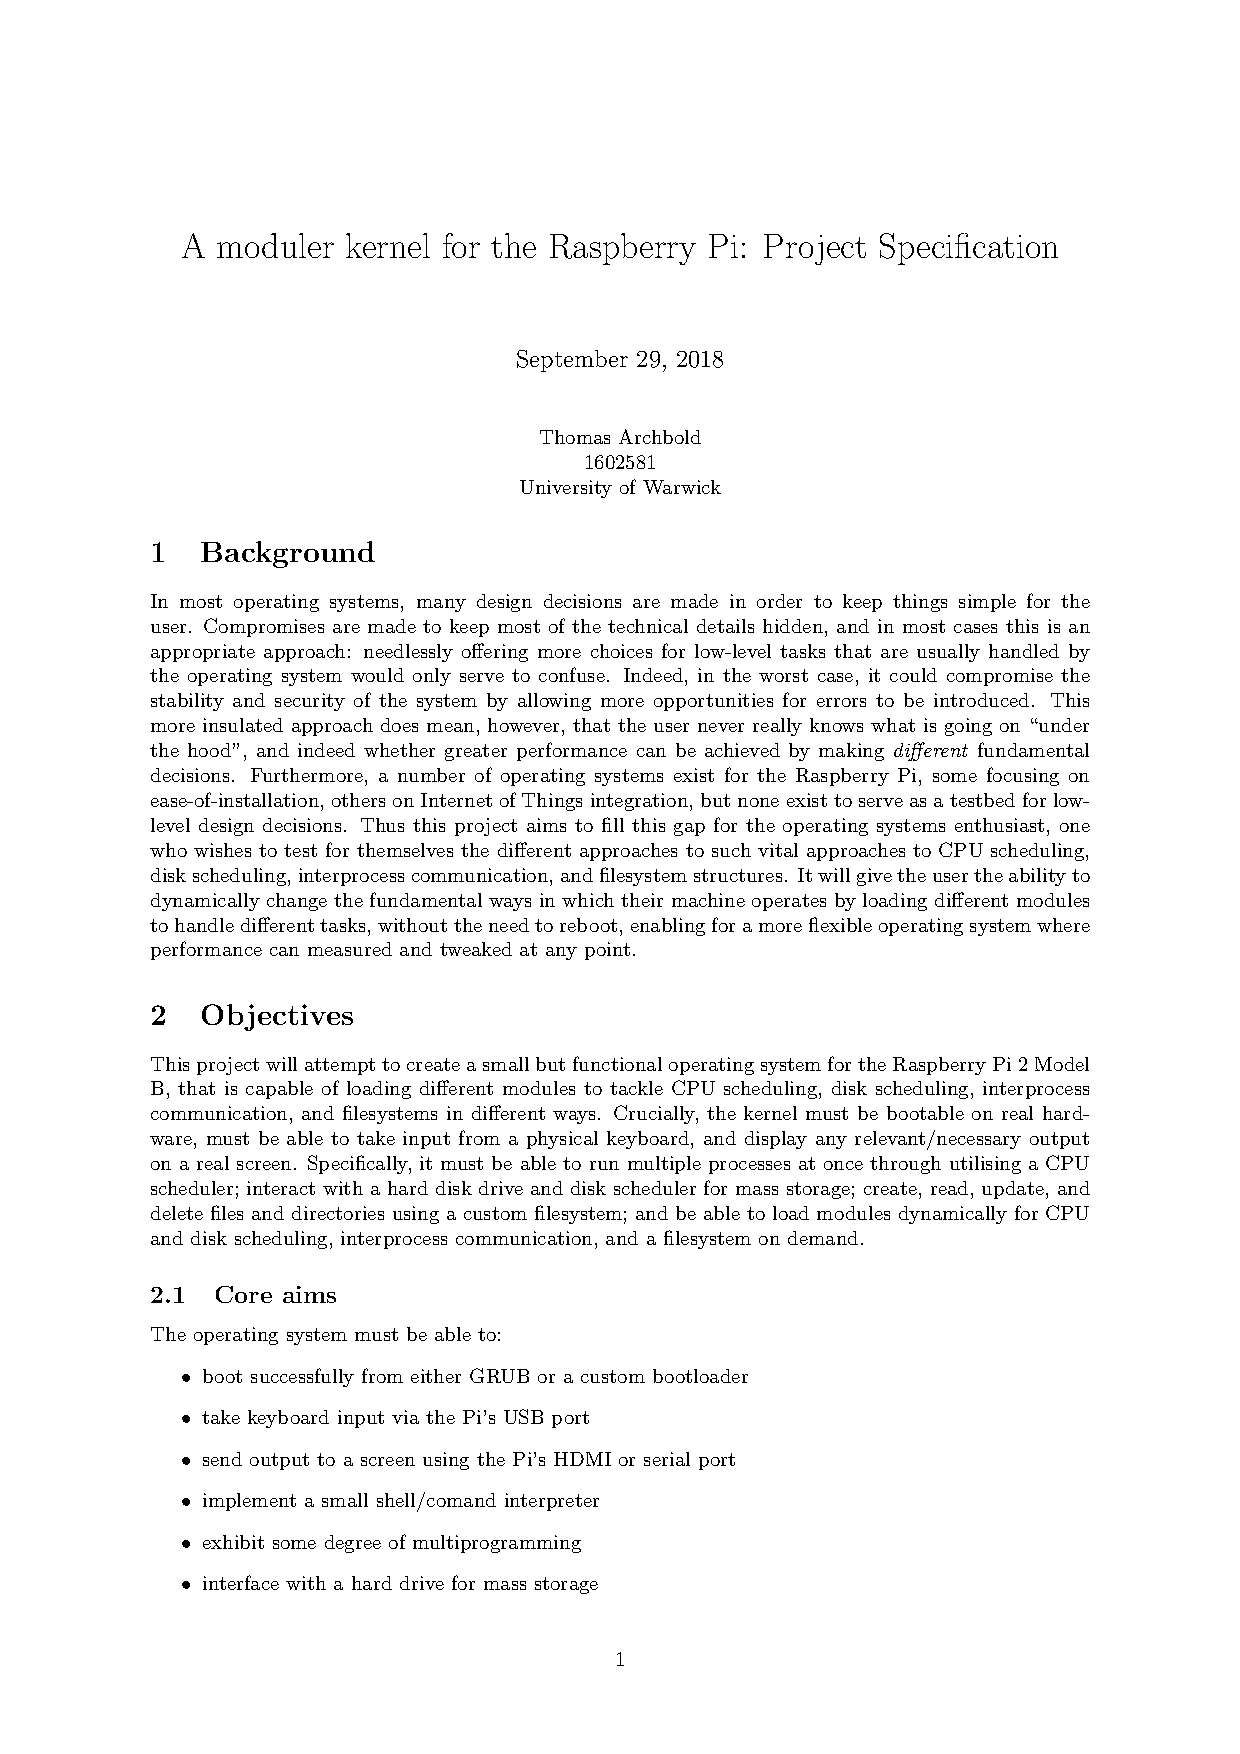
\includepdf[pages=-]{../specification/specification.pdf}

\end{appendices}

\end{document}
